\documentclass{article}

\usepackage{feynmp}
\usepackage{graphicx} %graphics
\usepackage{epstopdf} %EPS files
\usepackage{subfig} %figures with multiple parts
\usepackage{array} %for aligning table text in the middle
\usepackage{url} %properly formatted URLs
\usepackage{color}
\usepackage{amssymb}
\usepackage{mathtools}
\usepackage{subfiles} %to compile chapters individually in separate files
%\usepackage[justification=justified]{caption}[2009/9/16]
\usepackage[top=1in, bottom=1in, left=1.5in, right=1in]{geometry} %margins
\usepackage{setspace} %line spacing
\usepackage{multirow}
\usepackage{hyperref} %bibliography

%to get the subfloat references in 1(a) format instead of 1a
\DeclareSubrefFormat{myparens}{#1(#2)}
\captionsetup[subfloat]{subrefformat=myparens}

\frenchspacing %same spacing between words and sentences cf. http://en.wikibooks.org/wiki/LaTeX/Formatting#Space_between_Words_and_Sentences
\doublespacing %double spacing cf. http://en.wikibooks.org/wiki/LaTeX/Customizing_LaTeX#Spacing

%page numbering--needs to be top right, not yet working
\pagestyle{myheadings}
\markright{\hfill}

%shortcuts
\newcommand{\MET}{$\not\!\! E_{T}$ }
\newcommand{\ET}{$\mbox{E}_{\mbox{T}}$ }
\newcommand{\pT}{$\mbox{p}_{\mbox{T}}$ }
\newcommand{\NLSP}{\widetilde{\chi}_{1}^{0}}
\DeclareMathOperator{\sgn}{sgn}

%to interpret .1 file as .eps
\DeclareGraphicsRule{*}{mps}{*}{}

\begin{document}

\unitlength = 1mm

%qg-->qg (1 3g vertex, 1 qg vertex)
\begin{fmffile}{qg_to_qg_1}
\begin{fmfgraph*}(40,25)
\fmfleft{i1,i2}
\fmfright{o1,o2}
\fmflabel{$q$}{i1}
\fmflabel{$g$}{i2}
\fmflabel{$q$}{o1}
\fmflabel{$g$}{o2}
\fmf{fermion}{i1,v1,o1}
\fmf{curly}{i2,v2,o2}
\fmf{curly,label=$g$}{v1,v2}
\end{fmfgraph*}
\end{fmffile}
\vspace{1in}

%qg-->qg (2 qg vertices)
\begin{fmffile}{qg_to_qg_2}
\begin{fmfgraph*}(40,25)
\fmfleft{i1,i2}
\fmfright{o1,o2}
\fmflabel{$q$}{i1}
\fmflabel{$g$}{i2}
\fmflabel{$g$}{o1}
\fmflabel{$q$}{o2}
\fmf{fermion}{i1,v1}
\fmf{curly}{v1,o1}
\fmf{curly}{i2,v2}
\fmf{fermion}{v2,o2}
\fmf{fermion,label=$q$}{v1,v2}
\end{fmfgraph*}
\end{fmffile}
\vspace{1in}

%gg-->gg
\begin{fmffile}{gg_to_gg}
\begin{fmfgraph*}(40,25)
\fmfleft{i1,i2}
\fmfright{o1,o2}
\fmflabel{$g$}{i1}
\fmflabel{$g$}{i2}
\fmflabel{$g$}{o1}
\fmflabel{$g$}{o2}
\fmf{curly}{i1,v1,i2}
\fmf{curly}{o1,v2,o2}
\fmf{curly,label=$g$,label.dist=4mm}{v1,v2}
\end{fmfgraph*}
\end{fmffile}
\vspace{1in}

%qg-->qa
\begin{fmffile}{qg_to_qa}
\begin{fmfgraph*}(40,25)
\fmfleft{i1,i2}
\fmfright{o1,o2}
\fmflabel{$q$}{i1}
\fmflabel{$g$}{i2}
\fmflabel{$\gamma$}{o1}
\fmflabel{$q$}{o2}
\fmf{fermion}{i1,v1}
\fmf{photon}{v1,o1}
\fmf{curly}{i2,v2}
\fmf{fermion}{v2,o2}
\fmf{fermion,label=$q$}{v1,v2}
\end{fmfgraph*}
\end{fmffile}
\vspace{1in}

%qq-->aa
\begin{fmffile}{qq_to_aa}
\begin{fmfgraph*}(40,25)
\fmfleft{i1,i2}
\fmfright{o1,o2}
\fmflabel{$q$}{i1}
\fmflabel{$\bar{q}$}{i2}
\fmflabel{$\gamma$}{o1}
\fmflabel{$\gamma$}{o2}
\fmf{fermion}{i1,v1}
\fmf{photon}{v1,o1}
\fmf{fermion}{v2,i2}
\fmf{photon}{v2,o2}
\fmf{fermion,label=$q$}{v1,v2}
\end{fmfgraph*}
\end{fmffile}
\vspace{1in}

%gg-->aa
\begin{fmffile}{gg_to_aa}
\begin{fmfgraph*}(40,25)
\fmfleft{i1,i2}
\fmfright{o1,o2}
\fmflabel{$g$}{i1}
\fmflabel{$g$}{i2}
\fmflabel{$\gamma$}{o1}
\fmflabel{$\gamma$}{o2}
\fmf{curly}{i1,v1}
\fmf{curly}{i2,v3}
\fmf{fermion,label=$q$,label.side=right}{v1,v2,v4,v3,v1}
\fmf{photon}{v2,o1}
\fmf{photon}{v4,o2}
\end{fmfgraph*}
\end{fmffile}
\vspace{1in}

%qq-->Z-->qq-->qqa
\begin{fmffile}{qq_to_Z_to_qq_to_qqa}
\begin{fmfgraph*}(40,25)
\fmfleft{i1,i2}
\fmfright{o1,o2,o3}
\fmflabel{$q$}{i1}
\fmflabel{$\bar{q}$}{i2}
\fmflabel{$q$}{o1}
\fmflabel{$\bar{q}$}{o2}
\fmflabel{$\gamma$}{o3}
\fmf{fermion}{i1,v1}
\fmf{fermion}{v1,i2}
\fmf{photon,label=$Z$}{v1,v2}
\fmf{fermion}{v2,v3}
\fmf{fermion}{v3,o2}
\fmf{photon,tension=0}{v3,o3}
\fmf{fermion,tension=0.2}{o1,v2}
\end{fmfgraph*}
\end{fmffile}
\vspace{1in}

%qg-->qZ-->qff-->qffa
\begin{fmffile}{qg_to_qZ_to_qff_to_qffa}
\begin{fmfgraph*}(40,25)
\fmfleft{i1,i2}
\fmfright{o1,o2,o3,o4}
\fmflabel{$q$}{i1}
\fmflabel{$g$}{i2}
\fmflabel{$f^{-}$}{o1}
\fmflabel{$f^{+}$}{o2}
\fmflabel{$\gamma$}{o3}
\fmflabel{$q$}{o4}
\fmf{fermion}{i1,v1}
\fmf{curly}{i2,v2}
\fmf{fermion}{v2,o4}
\fmf{photon,label=$Z$}{v1,v3}
\fmf{fermion,label=$q$}{v1,v2}
\fmf{fermion,tension=0.2}{v3,o1}
\fmf{fermion}{v4,v3}
\fmf{fermion}{o2,v4}
\fmf{photon,tension=0}{v4,o3}
\end{fmfgraph*}
\end{fmffile}
\vspace{1in}

%qq-->W-->enu-->enua
\begin{fmffile}{qq_to_W_to_enu_to_enua}
\begin{fmfgraph*}(40,25)
\fmfleft{i1,i2}
\fmfright{o1,o2,o3}
\fmflabel{$q$}{i1}
\fmflabel{$\bar{q}^{'}$}{i2}
\fmflabel{$\nu_{e}$}{o1}
\fmflabel{$e$}{o2}
\fmflabel{$\gamma$}{o3}
\fmf{fermion}{i1,v1}
\fmf{fermion}{v1,i2}
\fmf{photon,label=$W$}{v1,v2}
\fmf{fermion}{v2,v3}
\fmf{fermion}{v3,o2}
\fmf{photon,tension=0}{v3,o3}
\fmf{fermion,tension=0.2}{o1,v2}
\end{fmfgraph*}
\end{fmffile}
\vspace{1in}

%qg-->qW-->qenu
\begin{fmffile}{qg_to_qW_to_qenu}
\begin{fmfgraph*}(40,25)
\fmfleft{i1,i2}
\fmfright{o1,o2,o3}
\fmflabel{$q$}{i1}
\fmflabel{$g$}{i2}
\fmflabel{$\nu_{e}$}{o1}
\fmflabel{$e$}{o2}
\fmflabel{$\bar{q}^{'}$}{o3}
\fmf{fermion}{i1,v1}
\fmf{curly}{i2,v2}
\fmf{fermion}{v2,o3}
\fmf{photon,label=$W$,label.side=right}{v1,v3}
\fmf{fermion,label=$\bar{q}^{'}$}{v1,v2}
\fmf{fermion,tension=0.2}{v3,o1}
\fmf{fermion}{o2,v3}
\end{fmfgraph*}
\end{fmffile}
\vspace{1in}

%gg-->tt-->WbWb-->ffbenub-->ffbenuba
\begin{fmffile}{gg_to_tt_to_WbWb_to_ffbenub_to_ffbenuba}
\begin{fmfgraph*}(80,50)
\fmfleft{i1,i2}
\fmfright{o1,o2,o3,o4,o5,o6,o7}
\fmflabel{$g$}{i1}
\fmflabel{$g$}{i2}
\fmflabel{$\bar{f}^{'}$}{o1}
\fmflabel{$f$}{o2}
\fmflabel{$b$}{o3}
\fmflabel{$\bar{b}$}{o4}
\fmflabel{$e^{+}$}{o5}
\fmflabel{$\gamma$}{o6}
\fmflabel{$\nu_{e}$}{o7}
\fmf{curly}{i1,v1,i2}
\fmf{fermion}{o3,v3}
\fmf{fermion,label=$\bar{t}$,label.side=left}{v3,v4}
\fmf{fermion,label=$t$}{v4,v5}
\fmf{fermion}{v5,o4}
\fmf{curly,label=$g$,label.dist=4mm}{v1,v4}
\fmf{photon,label=$W^{+}$,label.side=left}{v5,v7}
\fmf{photon,label=$W^{-}$}{v3,v2}
\fmf{fermion}{o1,v2,o2}
\fmf{fermion}{o5,v6}
\fmf{fermion}{v6,v7}
\fmf{photon,tension=0}{v6,o6}
\fmf{fermion}{v7,o7}
\end{fmfgraph*}
\end{fmffile}

%\begin{figure}
%	\centering
%	\subfloat{\label{fig:qg_to_qg_1}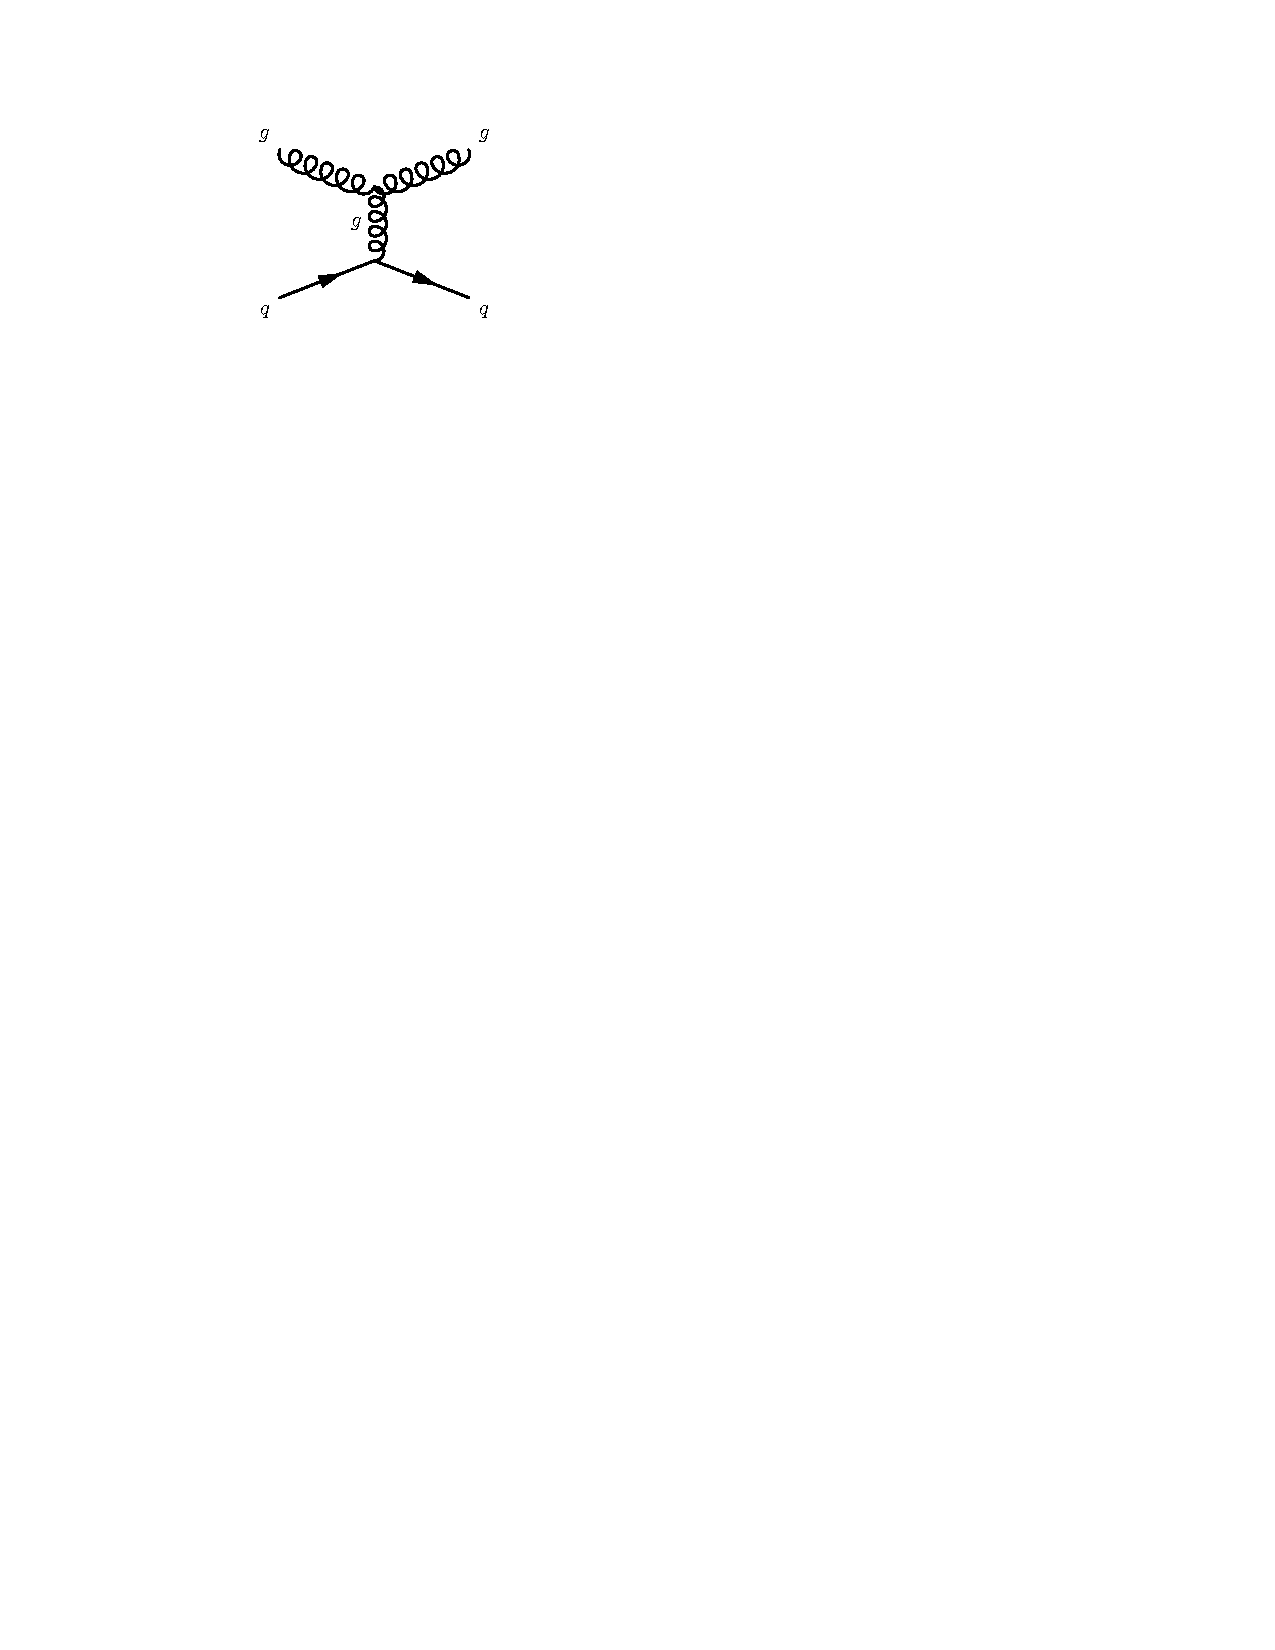
\includegraphics[scale=1.0]{qg_to_qg_1}}
%	\hspace{1cm}
%	\subfloat{\label{fig:qg_to_qg_2}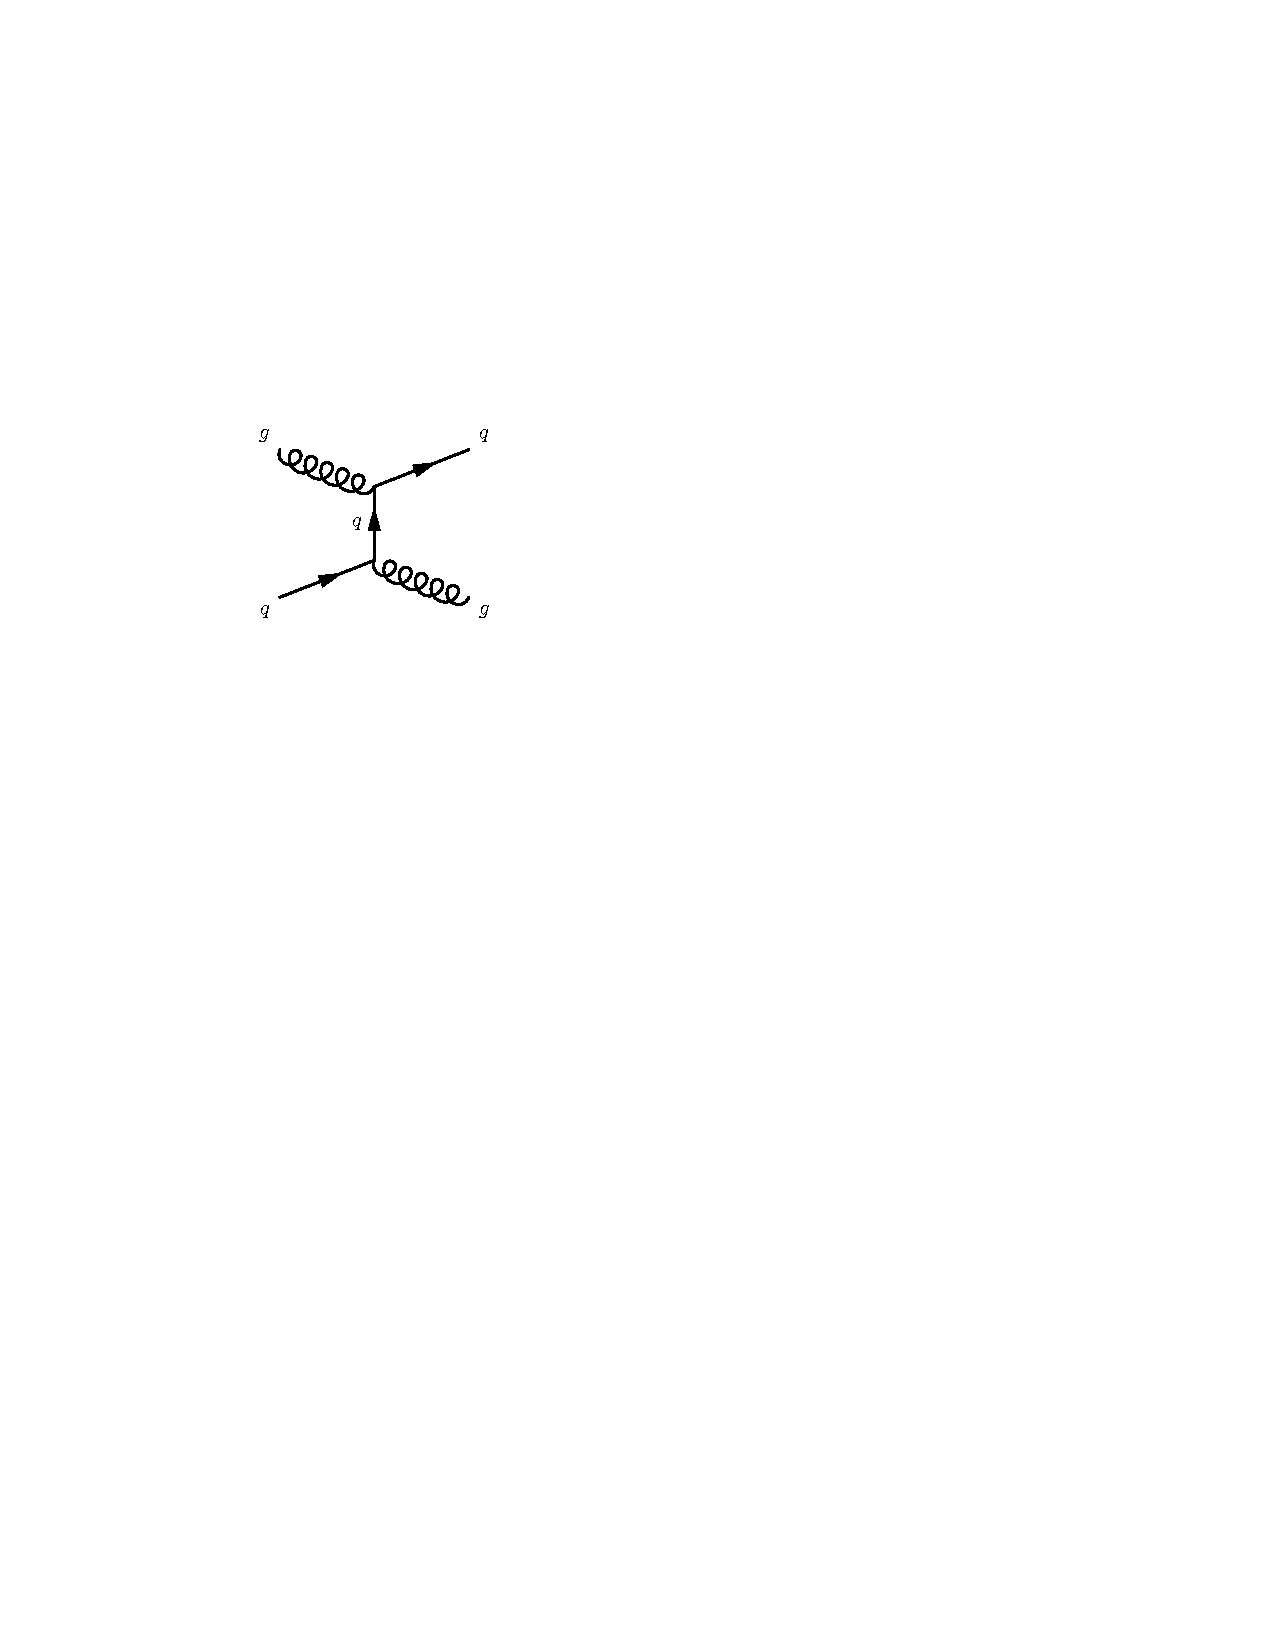
\includegraphics[scale=1.0]{qg_to_qg_2}}
%	\hspace{1cm}
%	\subfloat{\label{fig:gg_to_gg}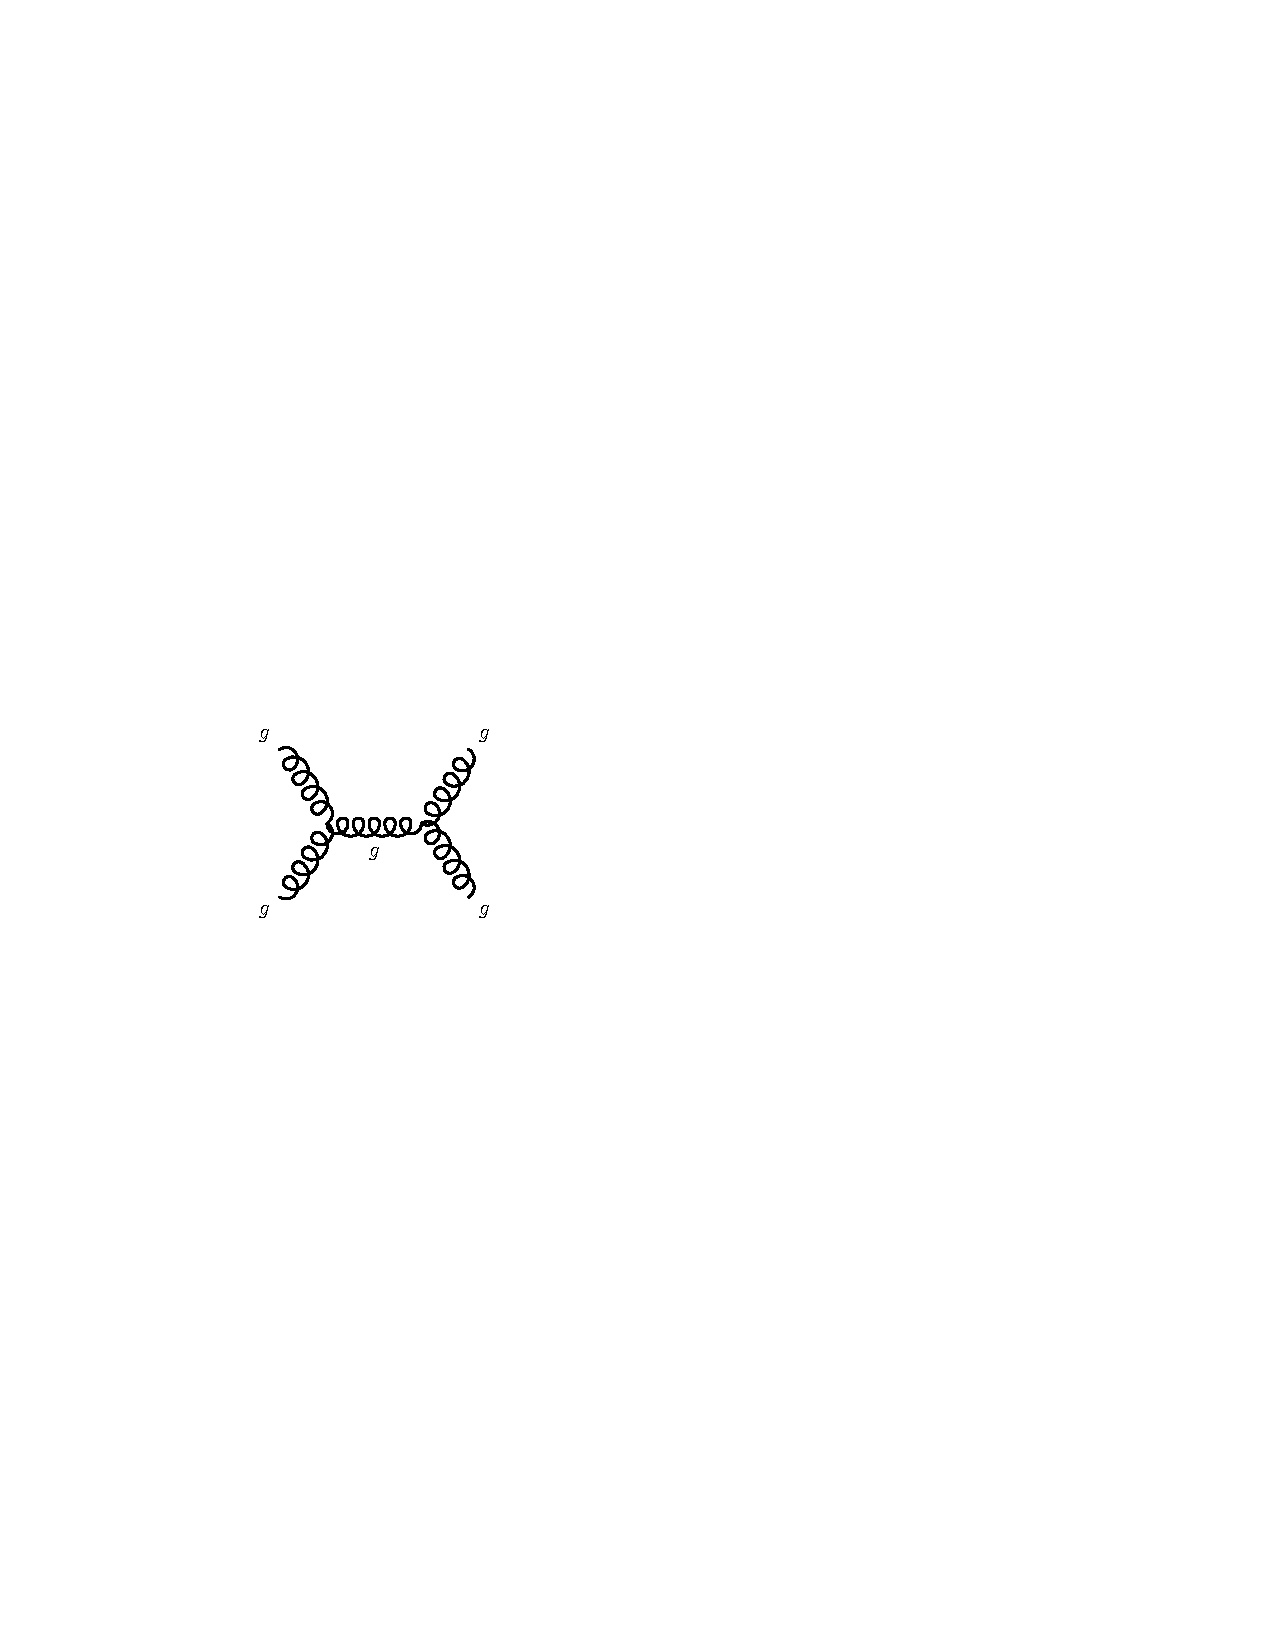
\includegraphics[scale=1.0]{gg_to_gg}}
%	\label{fig:dijet}
%\end{figure}
%
%\begin{figure}
%	\centering
%	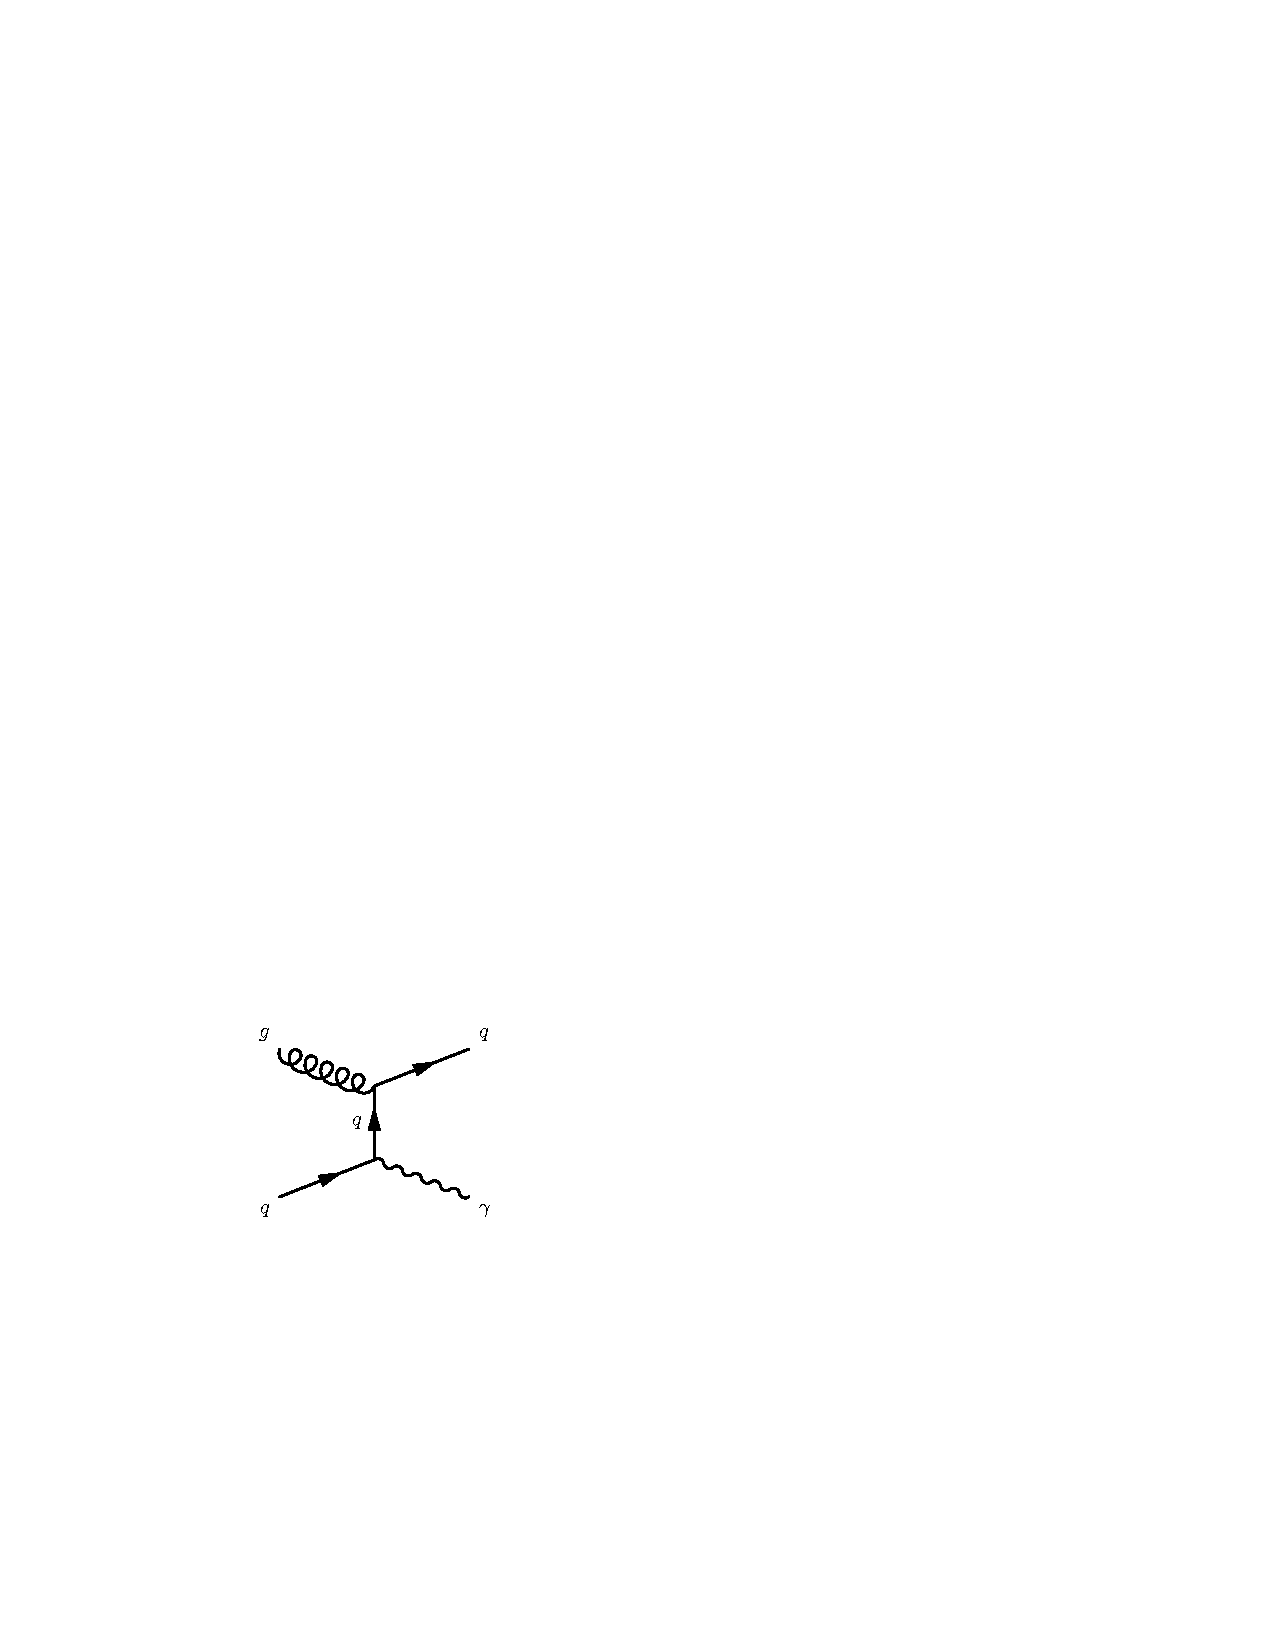
\includegraphics[scale=1.0]{qg_to_qa}
%	\label{fig:photon_jet}
%\end{figure}
%
%\begin{figure}
%	\centering
%	\subfloat{\label{fig:qq_to_aa}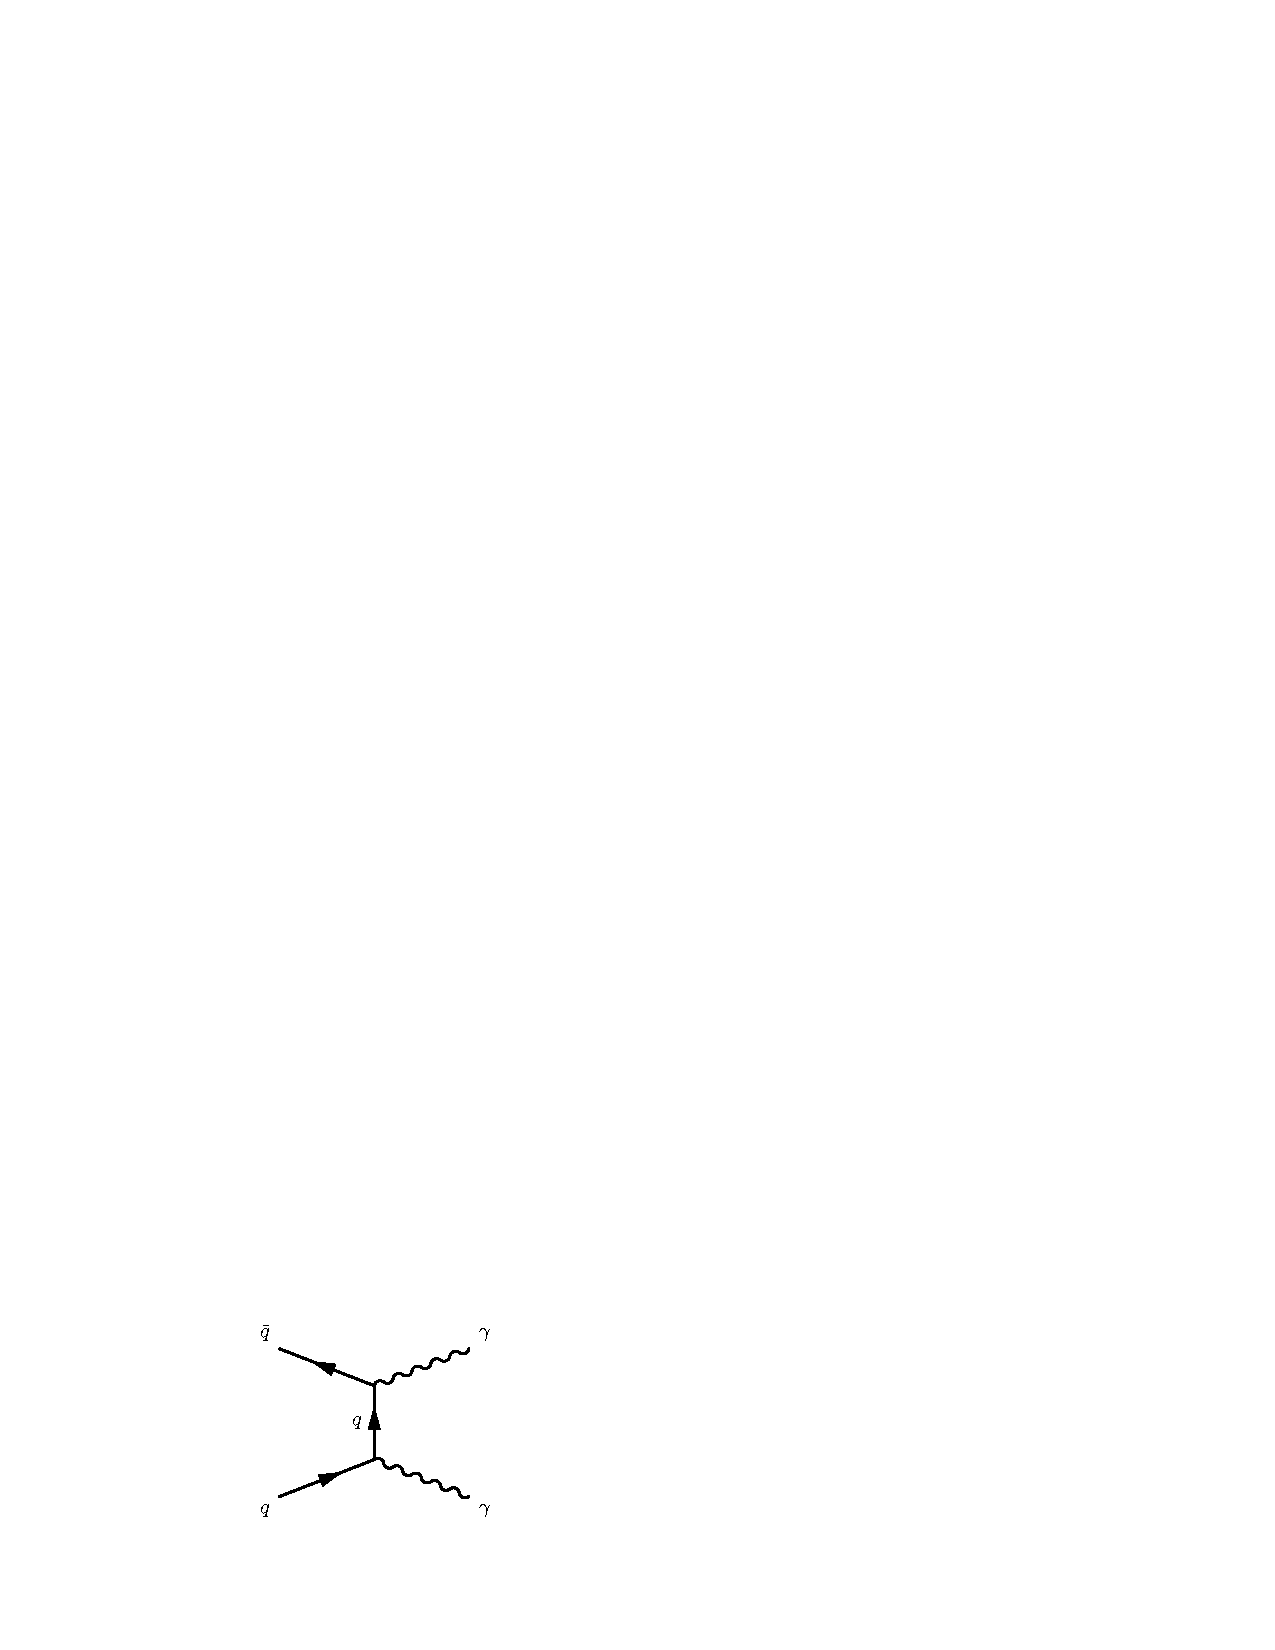
\includegraphics[scale=1.0]{qq_to_aa}}
%	\hspace{1cm}
%	\subfloat{\label{fig:gg_to_aa}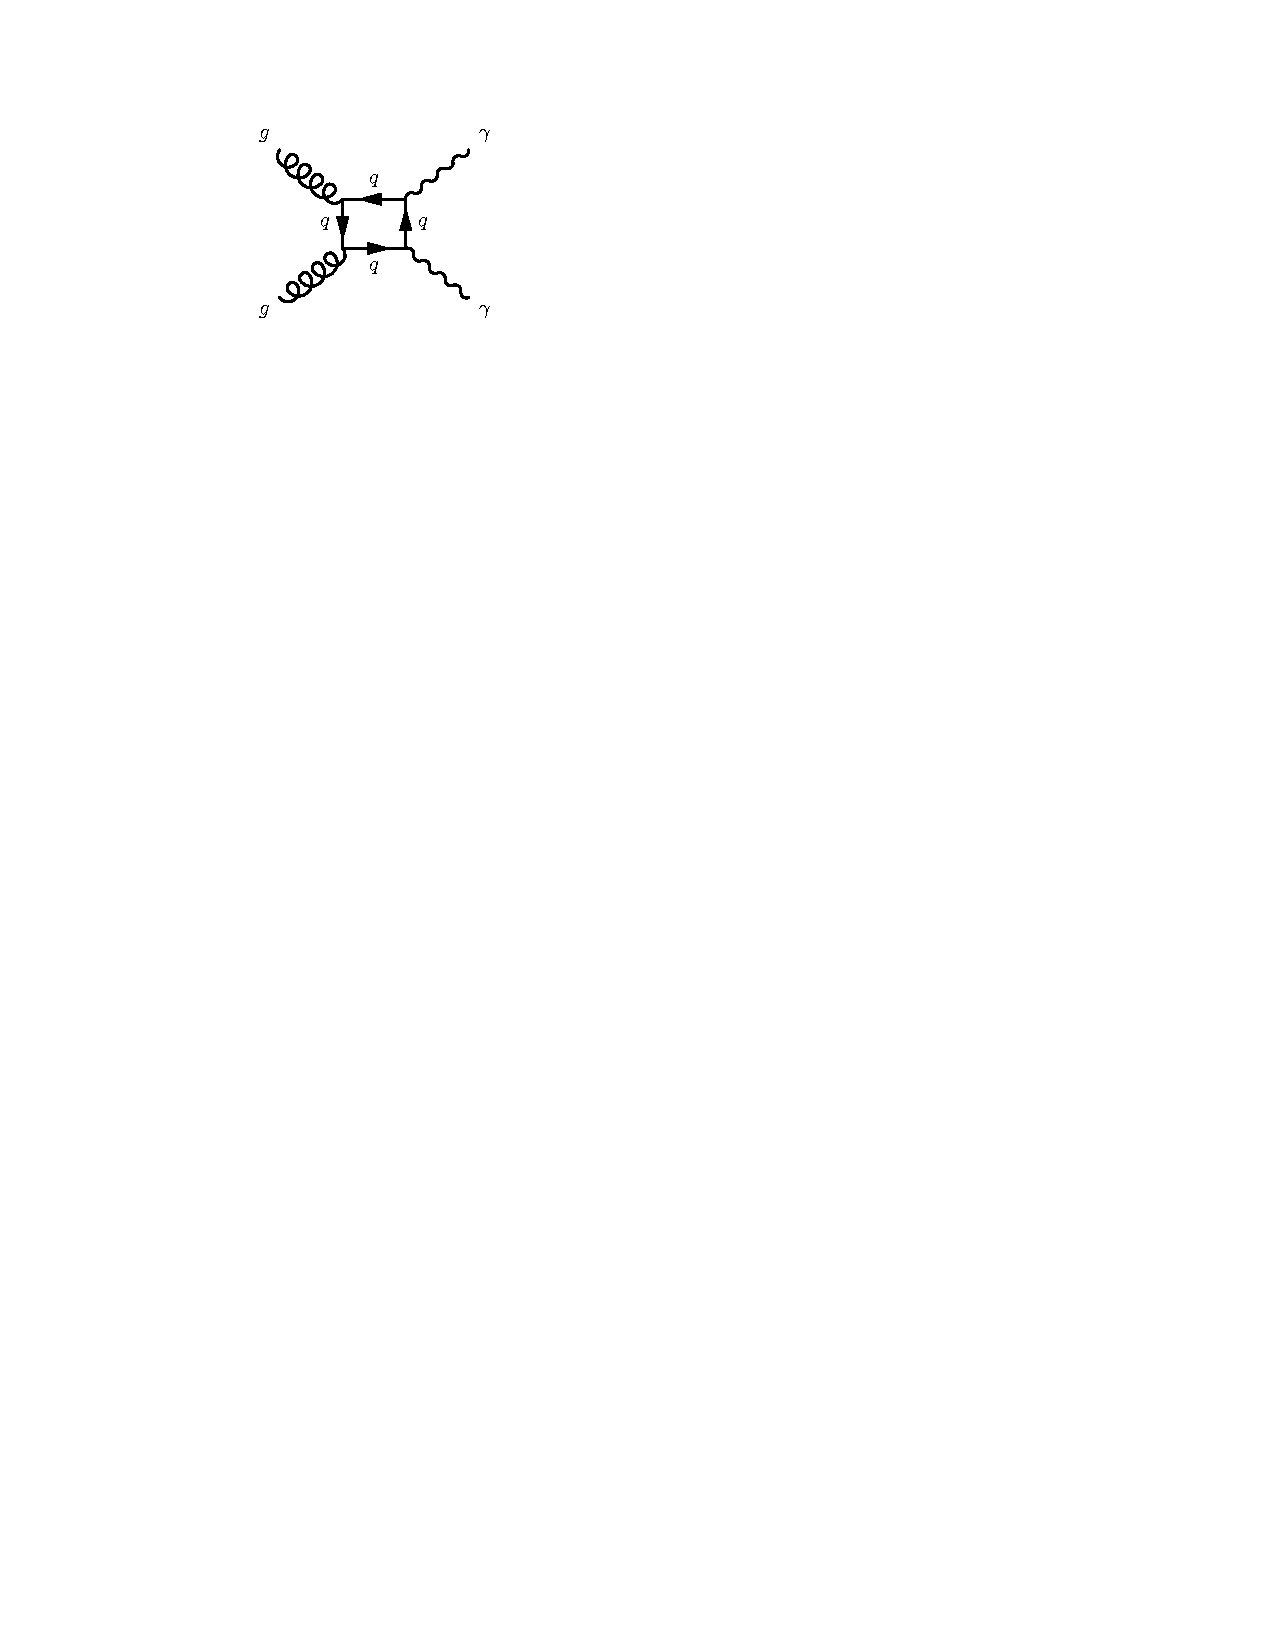
\includegraphics[scale=1.0]{gg_to_aa}}
%	\label{fig:diphoton}
%\end{figure}
%
%\begin{figure}
%	\centering
%	\subfloat{\label{fig:qq_to_Z_to_ee_to_eea}\includegraphics[scale=1.0]{qq_to_Z_to_ee_to_eea}}
%	\hspace{1cm}
%	\subfloat{\label{fig:qg_to_qZ_to_qee_to_qeea}\includegraphics[scale=1.0]{qg_to_qZ_to_qee_to_qeea}}
%	\label{fig:Zgamma}
%\end{figure}
%
%\begin{figure}
%	\centering
%	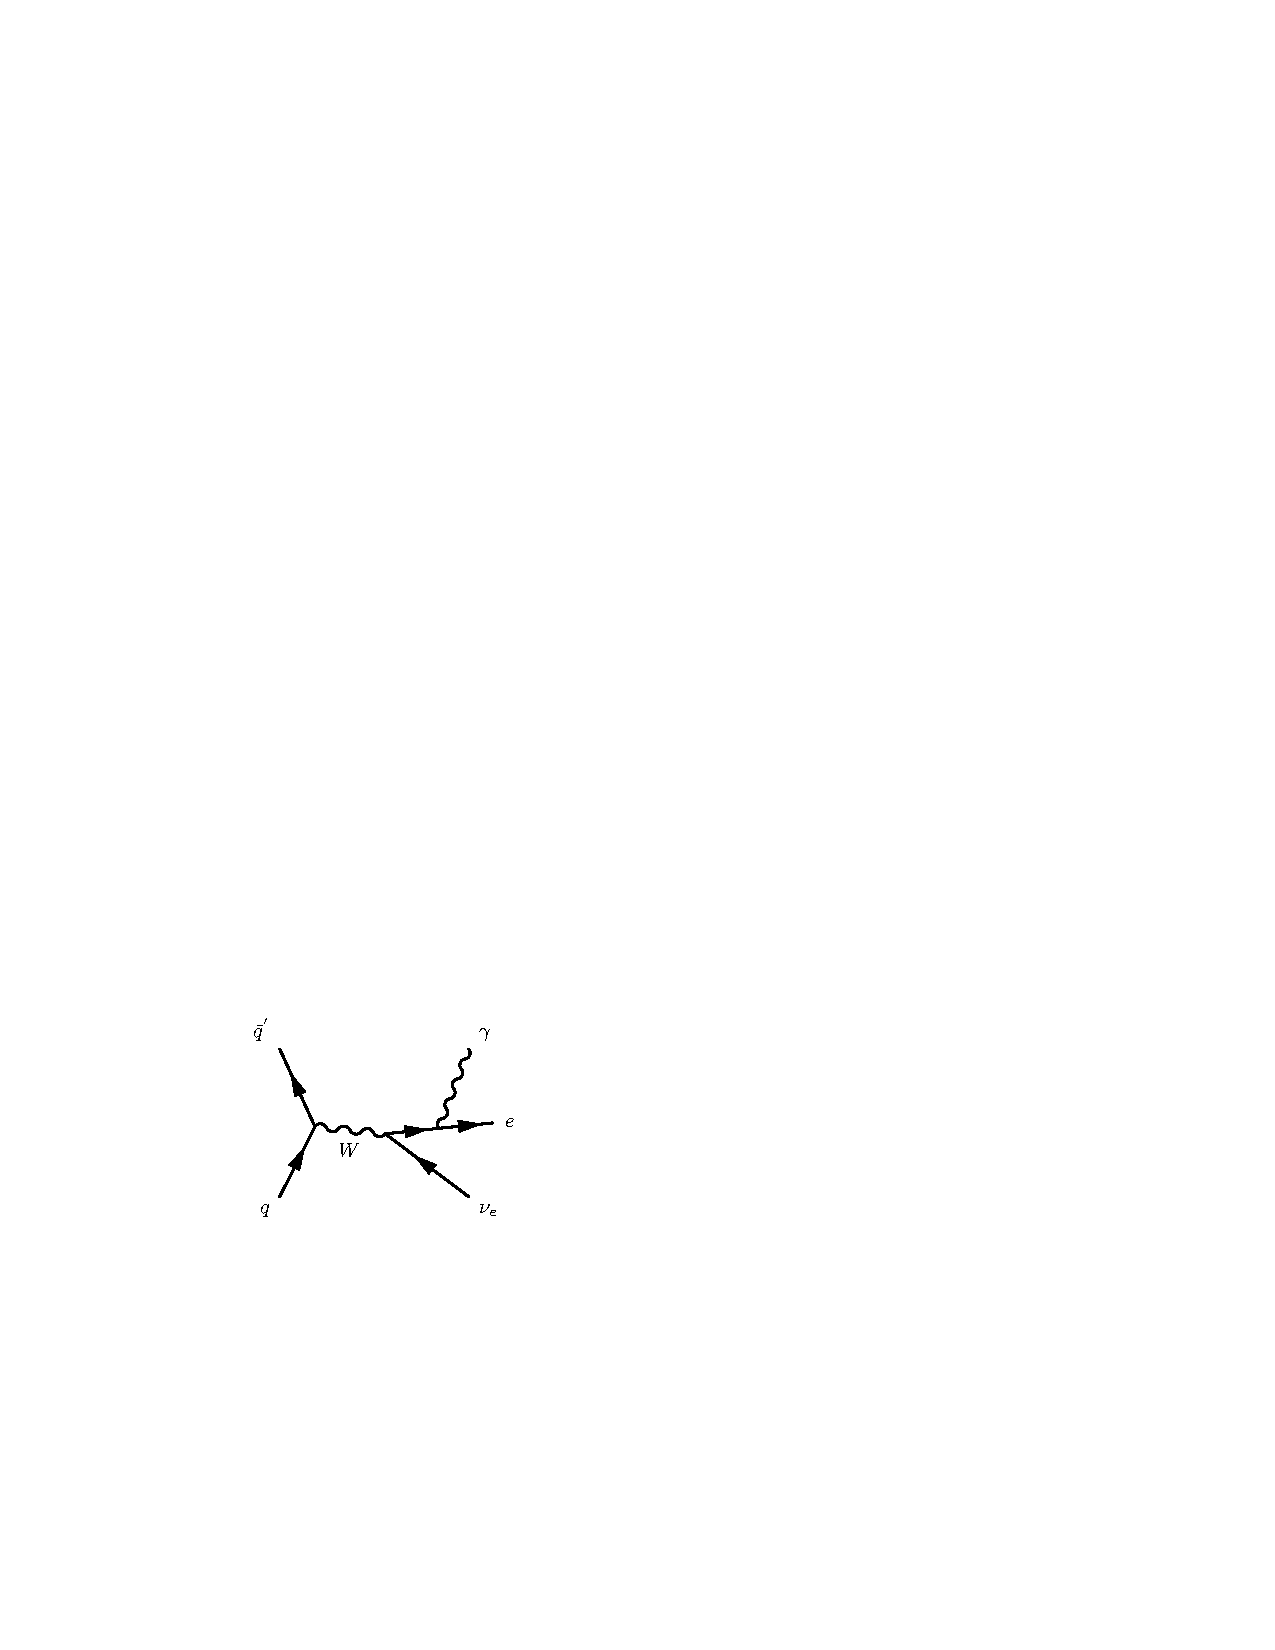
\includegraphics[scale=1.0]{qq_to_W_to_enu_to_enua}
%	\label{fig:Wgamma}
%\end{figure}
%
%\begin{figure}
%	\centering
%	\includegraphics[scale=1.0]{qg_to_qW_to_qenu_to_qenua}
%	\label{fig:W_jet}
%\end{figure}
%
%\begin{figure}
%	\centering
%	\includegraphics[scale=1.0]{gg_to_tt}
%	\label{fig:ttbar}
%\end{figure}

\end{document}